
A gesture recognition system can in many ways be regarded as a pipeline with three fundamental phases: Detection, tracking and recognition~\citep{Rautaray2015}.

% This section will describe what makes up a gesture recognition system, with special emphasis on hand gesture recognition, and
% summarize some common challenges with vision-based gesture recognition methods.

\subsection{Detection}
The first step in a typical gesture recognition system is to detect the relevant parts of the captured image and segment them from the rest. 
This segmentation is crucial because it isolates the relevant parts of the image from the background to ensure that only the relevant part is processed by the subsequent 
tracking and recognition stages~\citep{Cote2006}. 
A gesture recognition system will typically be interested in hand gestures, head- and arm movements and body poses, and thus only these factors should be observed by the system.
A gesture recognition system interested in detecting e.g.~hand gestures should thus only consider hands as a relevant segment, and thus only observe these.

Many different detection methods have been proposed by research, each using different visual features to detect relevant segments. 
Example of such visual features include skin color, shape, motion and anatomical models of the hands~\citep{Cote2006}.

\subsubsection{Color Detection} 
Color detection is a method of detecting the relevant segment (e.g.~hands) by its color. 
When employing this method one important decision is what color space to use, though color spaces efficiently separating the chromaticity from
the luminance components of color are typically the preferred ones. These are favored as they have some degree of robustness to illumination variability, which
is a weakness of this detection method. In addition to this skin color detection also have performance problems when the background contains objects that have a 
color distribution similar to human skin, although this can be combated by \textit{background subtraction}, and with variability in human skin tones~\citep{Rautaray2015}.

\subsubsection{Shape Detection} 
Shape detection is a method of detecting the relevant segment by its shape, and usually tries to extract the contours of objects to judge
whether those objects are relevant or not. An advantage with this method over color detection is that it's not directly dependent on skin color or
illumination, although these are still a factor~\citep{Rautaray2015}. However, a major disadvantage with this methods relates to occlusion and viewpoint
problems, which might cause a hand to not be recognized as one because of the camera angle and/or the hands orientation and configuration. One way to prevent this
might be to use several cameras with different viewpoints.
Shadows can also cause a problem as shadows of a hand often will be detected as hands themselves. Because of these disadvantages it is more
common to use this method in combination with other ones rather than on its own.

\subsubsection{Motion Detection} 
Motion detection is a method of detecting the relevant segment though motion, and assumes that all moving object are relevant.
When used as a gesture recognition scheme it requires a very controlled setup as it assumes that the only motion in the image is caused by hand movement. 
This method is also more commonly used in combination with other methods.

\begin{figure}%[h!] %[H]
	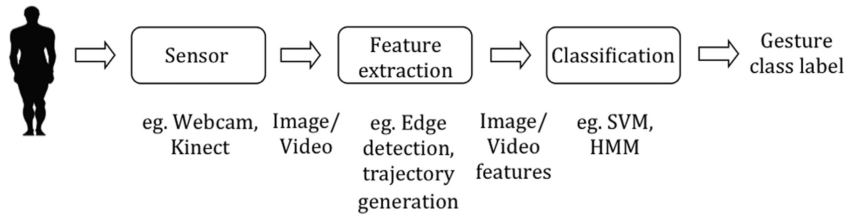
\includegraphics[width=\linewidth]{pictures/gr_pipeline.png}
	\caption[The gesture recognition pipeline]{A typical gesture recognition pipeline~\citep{Pisharady2015} }
	\label{fig:gr_pipeline}
\end{figure}

\subsection{Tracking}
The second step in a gesture recognition system is to track the movements of the relevant segments of the frames, e.g.~the hands. 
Tracking can be described as the frame-to-frame correspondence of the segmented hand regions and aims to understand the observed hand movements. 
This is often a difficult task as hands can move very fast and their appearance can change vastly within a few frames, 
especially when light conditions are a big factor~\citep{Wang2010}. 
One additional note is that if the detection method used is fast enough to operate at image acquisition frame rate, it can also be used for tracking~\citep{Rautaray2015}.   


\subsection{Recognition}
The last step of a gesture recognition system is to detect when a gesture occurs. 
This often implies checking against a predefined set of gestures, each entailing a specific action. 
To detect static gestures (i.e postures involving no movement) a general classifier or template-matcher can be used, 
but with dynamic gestures (which involves movement) other methods, which keep the temporal aspect, such as a Hidden Markov Model (HMM), are often required~\citep{Benton1995}. 
The recognition technology often makes uses of several methods from the field of machine learning, including supervised, unsupervised and reinforced learning.

When a gesture recognition system detects a relevant segment, it is thus tracked and represented in some way in the system. For hand gesture representations, 
which is the most relevant for this thesis, there are two major categories of hand gesture representations: 3D model-based methods and appearance-based methods~\citep{Rautaray2015}.

\begin{figure}%[h!] %[H]
	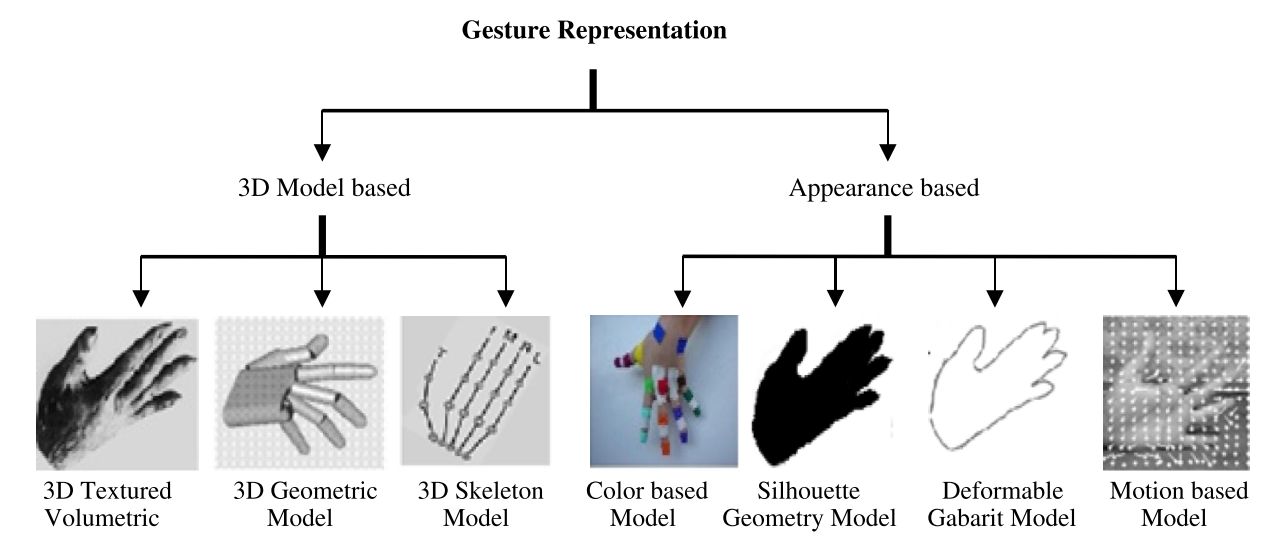
\includegraphics[width=\linewidth]{pictures/gesture_representation.png}
	\caption[Vision-based hand gesture representations]{Vision-based hand gesture representations~\citep{Bourke2007} }
	\label{fig:gesture_representations}
\end{figure}